\documentclass[border=4pt,12pt]{standalone}
% House style for redrawn exam diagrams (diagram-v4: 0.4pt lines, filled -latex arrows, fine dashes; stipple and hatching drawn as real dots/lines (no PDF/SVG patterns, so they render in every browser and at any scale); transparent background). Every figure \input's this.
\usepackage{amsmath,amssymb}
\usepackage{txfonts}
\usepackage{pdfrender,xcolor}
% \halo{text}: label on shading. The shading stops just around each letter's outline (a thin knock-out that follows the
% glyphs, like the papers' typesetting), never a box. Owner: "I don't want a box around the text".
\newcommand{\halo}[1]{\leavevmode\rlap{\pdfrender{TextRenderingMode=2,LineWidth=2.2pt,LineJoinStyle=1,StrokeColor=white,FillColor=white}#1}#1}
\usepackage{tikz,pgfplots}
\pgfplotsset{compat=1.18}
\usetikzlibrary{arrows.meta,calc,angles,quotes,patterns,patterns.meta,intersections,positioning,decorations.markings,shapes.geometric}
% Stipple and hatching are drawn as actual dots / lines clipped to the region (path picture), NOT as pattern fills:
% SVG <pattern> fills vanish or blur when browsers scale the image, so the owner could not see the shading.
% Each dot is a 0.72pt square (keeps SVGs small; reads as a dot at print size). Dots sit on one global staggered grid, so neighbouring regions line up.
\makeatletter
\newdimen\ex@x \newdimen\ex@y \newdimen\ex@xa \newdimen\ex@ya \newdimen\ex@xb \newdimen\ex@yb \newcount\ex@row
\def\exam@stipplecolor{black!75}\def\exam@dotr{0.42pt}\def\exam@dotgap{2.5}
\def\ex@rowdots{\ifdim\ex@x<\ex@xb \pgfpathrectangle{\pgfqpoint{\dimexpr\ex@x-0.36pt\relax}{\dimexpr\ex@y-0.36pt\relax}}{\pgfqpoint{0.72pt}{0.72pt}}\advance\ex@x by \exam@dotgap pt\relax\expandafter\ex@rowdots\fi}
\def\exam@stipple{%
  \pgftransformreset% dots are sized in real points even inside scaled pictures
  \pgfpointanchor{path picture bounding box}{south west}\ex@xa=\pgf@x \ex@ya=\pgf@y
  \pgfpointanchor{path picture bounding box}{north east}\ex@xb=\pgf@x \ex@yb=\pgf@y
  \pgfsetfillcolor{\exam@stipplecolor}\pgfmathsetmacro\ex@h{\exam@dotgap/2}%
  \pgfmathtruncatemacro\ex@r{floor(\ex@ya/\ex@h)-1}\ex@row=\ex@r\relax
  \ex@y=\ex@r\dimexpr\ex@h pt\relax
  \loop\ifdim\ex@y<\ex@yb
    \pgfmathtruncatemacro\ex@c{floor(\ex@xa/\exam@dotgap)-1}\ex@x=\ex@c\dimexpr\exam@dotgap pt\relax
    \ifodd\ex@row \advance\ex@x by \ex@h pt\fi
    \ex@rowdots
    \advance\ex@y by \ex@h pt \advance\ex@row by 1
    \ifnum\numexpr\ex@row-(\ex@row/4)*4\relax=0 \pgfusepath{fill}\fi% flush every 4 rows: bounded TeX memory, few clip copies in the SVG
  \repeat\pgfusepath{fill}}
\newdimen\ex@d
\def\exam@hatch#1{% #1 = 1 for /, -1 for \ ; lines 45 degrees, 3pt apart
  \pgftransformreset
  \pgfpointanchor{path picture bounding box}{south west}\ex@xa=\pgf@x \ex@ya=\pgf@y
  \pgfpointanchor{path picture bounding box}{north east}\ex@xb=\pgf@x \ex@yb=\pgf@y
  \ex@d=\dimexpr\ex@yb-\ex@ya\relax \ex@x=\dimexpr\ex@xa-\ex@d\relax
  \loop\ifdim\ex@x<\ex@xb
    \ifnum#1>0 \pgfpathmoveto{\pgfqpoint{\ex@x}{\ex@ya}}\pgfpathlineto{\pgfqpoint{\dimexpr\ex@x+\ex@d\relax}{\ex@yb}}%
    \else \pgfpathmoveto{\pgfqpoint{\ex@x}{\ex@yb}}\pgfpathlineto{\pgfqpoint{\dimexpr\ex@x+\ex@d\relax}{\ex@ya}}\fi
    \advance\ex@x by 4.24pt
  \repeat
  \pgfsetlinewidth{0.4pt}\pgfsetstrokecolor{black}\pgfusepath{stroke}}
\def\examstipple{\exam@stipple}\def\examhatch{\exam@hatch}\def\examsetstipplecolor#1{\def\exam@stipplecolor{#1}}\def\examsetdotgap#1{\def\exam@dotgap{#1}}
\makeatother
% (legacy pattern kept for old files)
% staggered stipple like the NESA papers' dotted shading
\pgfdeclarepatternformonly{exam stipple}{\pgfpointorigin}{\pgfqpoint{2.2pt}{2.2pt}}{\pgfqpoint{2.2pt}{2.2pt}}{%
  \pgfpathcircle{\pgfqpoint{0.55pt}{0.55pt}}{0.42pt}\pgfpathcircle{\pgfqpoint{1.65pt}{1.65pt}}{0.42pt}\pgfusepath{fill}}
\tikzset{
  every picture/.style={line width=0.6pt, >={Latex[length=2mm,width=1.3mm]}},
  curve/.style={line width=0.6pt},
  open arrow/.style={-{Latex[length=2mm,width=1.3mm]}},  % owner: filled -latex heads everywhere, no open chevrons
  aux/.style={dash pattern=on 2pt off 1.5pt, line width=0.6pt},
  shade/.code={\def\exA{#1}\def\exB{none}\ifx\exA\exB\else\pgfkeysalso{fill=black!18}\fi},
  shade/.default=on,
  shade dots/.style={fill=none, path picture={\examstipple}},
  stipple color/.code={\examsetstipplecolor{#1}},
  stipple gap/.code={\examsetdotgap{#1}},
  shade dense dots/.style={fill=none, stipple gap=1.6, path picture={\examstipple}},
  shade hatch/.style={fill=none, path picture={\examhatch{1}}},
  shade hatch reverse/.style={fill=none, path picture={\examhatch{-1}}},
  shade solid/.style={fill=black},
  pt/.style={circle, fill, inner sep=1.1pt},
  open pt/.style={circle, draw, fill=white, inner sep=1.1pt},
}
\pgfplotsset{
  exam axes/.style={axis lines=middle, axis line style={->}, xlabel={$x$}, ylabel={$y$},
    xlabel style={anchor=west}, ylabel style={anchor=south}, tick label style={font=\small},
    every axis plot/.append style={line width=0.6pt, black}, samples=200, clip=false,
    enlargelimits=false, axis on top},
}

\begin{document}
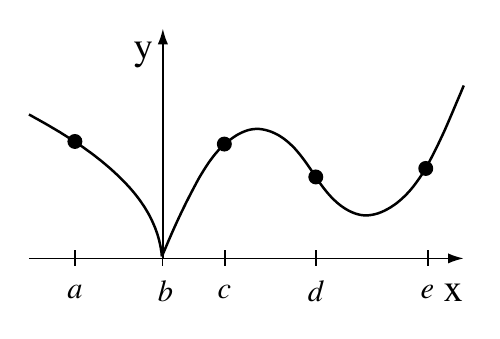
\begin{tikzpicture}[x=0.0127cm, y=-0.0127cm, font=\fontsize{11}{13}\selectfont]
  \draw[->] (20,254) -- (455,254);
  \draw[->] (154,254) -- (154,24);
  \foreach \x in {66,153.5,216,307,419} \draw (\x,246) -- (\x,262);
  \draw[smooth, line width=0.9pt] plot[smooth]coordinates {(20,110) (23.15,111.7) (26.29,113.5) (29.43,115.2) (32.56,117) (35.64,118.7) (38.76,120.5) (41.83,122.3) (44.88,124.1) (47.93,125.9) (50.96,127.7) (53.99,129.6) (57,131.5) (59.99,133.4) (62.93,135.2) (65.89,137.2) (68.84,139.2) (71.73,141.1) (74.64,143.1) (77.48,145.2) (80.31,147.2) (83.16,149.3) (85.94,151.4) (88.7,153.6) (91.43,155.7) (94.14,157.9) (96.83,160.2) (99.44,162.4) (102.1,164.7) (104.6,167) (107.2,169.4) (109.7,171.7) (112.2,174.2) (114.6,176.6) (117,179.1) (119.3,181.6) (121.6,184.1) (123.8,186.7) (126,189.3) (128.1,192) (130.1,194.6) (132.1,197.4) (133.9,200.1) (135.8,202.9) (137.5,205.7) (139.2,208.6) (140.8,211.5) (142.3,214.5) (143.7,217.5) (145,220.5) (146.3,223.5) (147.4,226.6) (148.5,229.7) (149.4,232.8) (150.3,236) (151,239.1) (151.7,242.3) (152.2,245.5) (152.7,248.7) (153,252)};
  \draw[smooth, line width=0.9pt] plot[smooth]coordinates {(153,252) (156.9,242.9) (160.7,234) (164.6,225.1) (168.6,216.3) (172.7,207.6) (176.9,199) (181.2,190.5) (185.6,182.1) (190,173.9) (194.7,166.1) (199.4,158.8) (204.4,152) (209.6,145.8) (215.1,140.3) (221.1,135.4) (227.2,131.1) (233.3,127.9) (239.2,125.7) (244.9,124.6) (250.6,124.5) (256.6,125.5) (262.7,127.4) (268.9,130.3) (274.8,134.1) (280.5,138.7) (286,144.1) (291.2,150.2) (296.5,157.2) (301.8,164.8) (307.2,172.9) (312.4,180.4) (317.6,187.1) (322.8,193) (328.4,198.3) (334.2,202.8) (340.2,206.4) (346.2,209) (351.8,210.5) (357.4,211) (363.2,210.4) (369.3,208.9) (375.8,206.2) (382.1,202.7) (388.3,198.4) (394.1,193.4) (399.7,187.8) (405,181.5) (409.9,174.8) (414.7,167.5) (419.2,159.7) (423.5,151.6) (427.7,143.3) (431.8,134.7) (435.8,126.1) (439.7,117.2) (443.5,108.3) (447.3,99.3) (451.2,90.17) (455,81)};
  \foreach \p in {(66,137),(215.5,139.6),(307,172.5),(417,164)} \fill \p circle (2.7pt);
  \node[font=\fontsize{14}{16}\selectfont] at (134.5,50) {y};
  \node[font=\fontsize{14}{16}\selectfont] at (444.5,288) {x};
  \foreach \x/\l in {66/a,156.5/b,215.5/c,307/d,418.5/e} \node at (\x,287) {$\l$};
\end{tikzpicture}
\end{document}
